\documentclass[12pt]{amsart}
\usepackage{amssymb}
\usepackage{stmaryrd}
\usepackage{graphicx}
\usepackage{todonotes}

\usepackage{tensor}

\newcommand{\hoj}[1]{\todo[inline,color=blue!20]{HOJ: #1}}
\newcommand{\cjc}[1]{\todo[inline,color=red!20]{CJC:  #1}}
\newcommand{\je}[1]{\todo[inline,color=green!20]{JE:  #1}}


\newcommand{\pder}[2]{\ensuremath{\frac{\partial #1}{\partial #2}}}
\newcommand{\so}{\ensuremath{\mathfrak{so}}}
\newcommand{\R}{\ensuremath{\mathbb{R}}}

\newtheorem{thm}{Theorem}[section]
\newtheorem{prop}[thm]{Proposition}
\newtheorem{lem}[thm]{Lemma}
\newtheorem{cor}[thm]{Corollary}
\newtheorem{defn}[thm]{Definition}

\DeclareMathOperator{\SDiff}{SDiff}
\DeclareMathOperator{\Diff}{Diff}
\DeclareMathOperator{\Jet}{Jet}
\DeclareMathOperator{\SO}{SO}
\DeclareMathOperator{\SL}{SL}
\DeclareMathOperator{\tr}{tr}
\DeclareMathOperator{\iso}{iso}
\DeclareMathOperator{\kernel}{kernel}
\DeclareMathOperator{\lie}{\mathcal{L}}

\title[A meshless method for ideal fluid flow derived from s.g.]{A meshless method for
 ideal fluid flow derived from symplectic geometry}

\author{Ronan}

\begin{document}
\maketitle

\begin{abstract}
  blah blah blah
\end{abstract}

\section{Introduction}
\hoj{Quickly describe the derivation of point-vortex solutions and peakons via Clebsch variables.
	Then describe out method.}

\subsection{Main contributions}
In this article we propose a hierarchy of particle methods
for a regularized model of ideal fluids.
These models will be derive via techniques from 
symplectic geometry and Hamiltonian mechanics.
The main contributions are:
\begin{enumerate}
  \item We determine Poisson morphism which constitute 
    dual-pairs that induce these methods.
  \item We relate the ``right-leg'' of the dual pairs to Kelvin's circulation theorem.
  \item We explore the collision behavior discovered in \cite{CotterHolmJacobsMeier2014}.
\end{enumerate}
As a ``softer'' contribution, we explain this method entirely in the Hamiltonian
formalism to provide an alternative perspective to previous works written in the Lagrangian formalism.\cjc{remove apology, move this contribution to front.}

\subsection{Previous work}
This article concerns a hierarchy of particle methods for
ideal incompressible fluids, which we have dubbed \emph{jetlet methods}.
The zeroth order jetlet method was first discovered in \cite{MumfordMichor2013}
where error bounds in comparison with solutions of Euler's equations were
calculated.
Simultaneously, foundational work for particle methods carrying Taylor series
data was developed in \cite{JacobsRatiuDesbrun2013}.
Based upon the foundational work of \cite{JacobsRatiuDesbrun2013},
an implementation using the fluid model of \cite{MumfordMichor2013} was created \cite{CotterHolmJacobsMeier2014}.
A primary finding of \cite{CotterHolmJacobsMeier2014} was that particle collisions at one level of the hierarchy can exhibit ``infinite time mergers'' into particles at higher-levels in the hierarchy. 
In both \cite{MumfordMichor2013} and \cite{CotterHolmJacobsMeier2014}, the
equations of motion were viewed as Euler--Lagrange equations
obtained from variational principles.
In particular, the insights one could glean from 
the Hamiltonian perspective were left untouched.

In this article we will use Poisson maps to determine solutions of regularized
fluid equations by solving finite dimensional Hamiltonian equations.
The notions of momentum maps and dual pairs are typically
regarded as notions of symplectic geometry \cite{FOM,Weinstein1983}.
However, many of the statements on momentum maps and
dual pairs in this article
have analogs in the Lagrangian perspective.
In particular, the dual pairs of the Camassa--Holm equation
first appeared in \cite{HolmMarsden2005}, where the Clebsch
variational principle was used to derive equations of motion.
Moreover, the Clebsch variational principle was used in
\cite{CotterHolm2009} in the context of optimal control.
Momentum maps were found to naturally arise when the
control vector fields form a subalgebra of the space of all
 vector fields.
 
 Here are other articles we should cite:
 \begin{enumerate}
 	\item \cite{MarsdenWeinstein1983,Weinstein1983} for dual pairs.
 	\item \cite{Chorin1973} for vortex method.
	\item \cite{Sommer2013,CotterHolmJacobsMeier2014} for jet particles
	\item \cite{HolmTronci2012} for particles carrying diffeomorphisms as advected quantity in a turbulence model.
 	\item \cite{JacobsRatiuDesbrun2013} for particle methods via Lagrange--Poincar\'e.
	\item \cite{FoiasHolmTiti2001} for convergence of NS-$\alpha$ to NS.
	\item \cite{Arnold1966} for Euler fluid as Euler--Poincar\'e on $\SDiff(\R^n)$.
	\item \cite{TrouveYounes2005} for analysis of particle methods for EP.
	\item Euler-$\alpha$ papers.
	\item One``Beg-algorithm" paper, such as \cite{Beg2005}.
	\item \cite{JoshiMiller2000} for particle methods for Beg algorithm.
	\item \cite{HoldenRaynaud2006} for particle method for CH via peakons.
	\item \cite{ChertockDuToitMarsden2012} for particle method for $n$-dimensional CH via peakons.
 \end{enumerate}
\todo[inline]{Finish this section.}

\subsection{Notation}
tangent bundle, cotangent bundle, vector field, contraction, Lie derivative,
smooth, continuous functions, group actions, infinitesimal generators,
dual spaces.  A group $G$, left multiplication $L_g$, right multi $R_g$, 
left/right action $\rho(g,x)$ or $\rho(x,g)$, infinitesimal generator $\rho(\xi,x)$ or $\rho(x,\xi)$.
\todo[inline]{Finish this section}

\section{Hamiltonian mechanics}
\label{sec:Hamiltonian}
The goal of this section is to prove theorems \ref{thm:dual_pairs}
and \ref{thm:commuting_actions} (see pages \pageref{thm:dual_pairs} and \pageref{thm:commuting_actions}).
Those who understand and accept these theorems on a first reading
should be able to skip this section without any consequence.
Most of this section will be a crash course in Poisson geometry
and Hamiltonian mechanics as described in \cite{FOM,MandS,Weinstein1983}.

A typical introduction to Poisson structures in mechanics
begins by considering Hamilton's equations
\begin{align*}
  \dot{q} = \pder{H}{p} \quad, \quad  \dot{p} = - \pder{H}{q}.
\end{align*}
If we consider the two-form $dp \wedge dq$, then Hamilton's equations
can be written as $(\dot{q},\dot{p}) \lrcorner (dp \wedge dq) = dH(q,p)$.
This is the starting point for symplectic geometry, which
will be discussed in \S \ref{sec:Symplectic}.
Alternatively, these equations can be written using the bilinear map $\{ \cdot , \cdot \}_{\rm can} : C^1( T^*Q) \times C^1(T^*Q) \to C^0(T^*Q)$
given by
\begin{align*}
  \{ F , G \}_{\rm can} = \pder{F}{q}\pder{G}{p} - \pder{G}{q} \pder{G}{p}.
\end{align*}
In particular, we may write $\dot{q} = \{ q , H \}_{\rm can}$ and $\dot{p} = \{ p , H\}_{\rm can}$.
The object $\{ \cdot , \cdot \}_{\rm can}$ is a special case of more general
object known as a \emph{Poisson bracket} which will be introduced in
\S \ref{sec:Poisson}.

As a warning, symplectic geometry has developed greatly
since its origins in mechanics, and
has branched into an independent subfield of pure mathematics.
Many notions were revised and optimized in the $1970$'s and $1980$'s for
the purpose of proving theorems.
Occasionally these revisions entailed a sacrifice
in clarity, from the perspective of ``outsiders''.
This paper is intended to allow ``outsiders''
(such as ourselves) to reap the benefits of Poisson geometry.
Therefore, we will cut away as much abstraction as possible in this introductory
section.
Nonetheless, a minimal amount of abstraction is needed in order to
maintain mathematical rigour and stand firmly upon the shoulders of giants.

\subsection{Symplectic manifolds}
\label{sec:Symplectic}
We begin with the definition.
\begin{defn}
  Let $S$ be a manifold
  and let $\omega$ be a closed two-form on $S$ such that the map
  ``$v \in TS \mapsto \omega( v , \cdot ) \in T^*S$'' is weakly nondegenerate.\footnote{
    A linear map $L:V \to V^*$ is \emph{weakly nondegenerate} if $L$ is injective.  If $V$ is finite dimensional, this simply means that $L$ is invertible.}
  We call $\omega$ a \emph{symplectic form}.
  We call the pair $(S,\omega)$ a \emph{symplectic manifold}.
\end{defn}
\je{Does this include infinite dimensional manifolds? Any
  notes/references on technical details?}
As a first example, consider the manifold $\R^2$
with coordinates $(q,p)$.
The two-form $dq \wedge dp$ is a symplectic form.
Given a manifold $Q$,
the cotangent bundle $T^*Q$ has local fiber bundle coordinates
given by $(q^1,\dots, q^n,p_1,\dots,p_n)$ and there is a unique symplectic form
which is locally expressed by $dp^i \wedge dq_i$, where
a sum on repeated indices is assumed.
This local expression corresponds to a global symplectic
form on $T^*Q$, known as the \emph{canonical symplectic form}
and denoted $\omega_{\rm can}$ \cite[Theorem 3.2.10]{FOM}.
In fact, given any symplectic manifold $(S,\omega)$, the dimension of $S$
is even, and there exist local coordinates $(q^1,\dots,q^n,p_1,\dots,p_n)$
such that $\omega \stackrel{locally}{=} dp_i \wedge dq^i$.
This is known as \emph{Darboux's theorem} and we call these type of
coordinates \emph{Darboux coordinates}\cite[Theorem 3.2.2]{FOM}.

Given a function $H:S \to \mathbb{R}$,
the exterior derivative is the one-form $dH:S \to T^*S$
expressed in local coordinates by $dH(x) = \pder{H}{x^i} dx^i$.
The Hamiltonian vector field $X_H:S \to TS$ is the unique vector
field defined by the condition
$
  X_H \lrcorner \omega = dH.
$
The symbol ``$\lrcorner$'' is the operation of contraction between
the contravariant indices of $X_H$ and the first set of covariant
indices of $\omega$.
In Darboux coordinates, the Hamiltonian vector field induces the
equations of motion $\dot{q}^i = \pder{H}{p_i}, \dot{p}_i = \pder{H}{q^i}$.


An important aspect of study in Hamiltonian mechanics is that of symmetry.
This yields the following notions

\begin{defn}
  Let $G$ be a Lie group and let $\rho:G \to \Diff(S)$ be a group action on a symplectic manifold $(S,\omega)$.
  The group $G$ is said to \emph{act symplectically}
  \begin{align*}
    \omega( \rho( g ) \cdot v , \rho(g) \cdot w) = \omega(v,w)
  \end{align*}
  for any $g \in G, v,w \in T_xS$ and $x \in S$.
  If $\mathfrak{g}$ is the Lie algebra of such a group,
  the \emph{momentum map}, $J:S \to \mathfrak{g}^*$,
  is defined by the property
  \begin{align*}
    d \langle J , \xi \rangle = \xi_S \lrcorner \omega.
  \end{align*}
\end{defn}

Alternatively, we can characterize a momentum map $J: S \to \mathfrak{g}^*$, as the unique map such that $X_{\langle J , \xi \rangle} = \xi_S$ for any $\xi \in \mathfrak{g}$.
In the special case where $S = T^*Q$, a left/right action of $G$ on $Q$ can be lifted to a right/left symplectic action on $T^*Q$ given by
\begin{align*}
  (q,p) \in T^*Q \mapsto (g^{-1} \cdot q , g^* p) \in T^*Q.
\end{align*}
where $g^*p$ is the unique covector such that $\langle g^*p , v \rangle = \langle p , Tg \cdot v \rangle$.
In this case the momentum map is characterized by the condition
\begin{align}
  \langle J(q,p) , \xi \rangle = \langle p , \xi \cdot q \rangle.
  \label{eq:cotangent_momap}
\end{align}
This is contained in Theorem 12.1.4 of \cite{MandS}.

Finally, given to functions $f,h \in C^{\infty}(S)$ we can consider the function $\{ f,h\} = \omega( X_f, X_h)$.
In Darboux coordinates $\{ f , h \} = \pder{f}{q^i} \pder{h}{p_i} - \pder{f}{p_i} \pder{h}{q^i}$.
Hamilton's equations can then be written as $\dot{q}^i = \{ q^i , h \},
\dot{p}_i = \{ p_i , h \}$.
We call $\{ \cdot , \cdot \}$ a Poisson bracket, and it is the subject of
the next subsection.

\subsection{Poisson manifolds}
\label{sec:Poisson}
We begin with the definition.

\begin{defn} \label{defn:Poisson}
  Let $P$ be a manifold, and $\{ \cdot , \cdot \}$ be a bilinear
  operation on $C^{\infty}(P)$ such that 
  $( C^{\infty}(P) , \{ \cdot , \cdot \} )$ is a Lie algebra
  and $\{ \cdot , h \}$ has the derivation property for any $h \in C^{\infty}(P)$.
  That is to say
  \begin{align*}
    \{ gf , h \} = \{ f , h \} \cdot g + \{ g , h \} \cdot f,
  \end{align*}
  for any $f,g,h \in C^{\infty}(P)$.
  We call $\{ \cdot , \cdot \}$ a \emph{Poisson bracket},
  and we call the pair $(P, \{ \cdot , \cdot \})$ a Poisson manifold.
\end{defn}

The first most important example of a Poisson bracket is
that of a Poisson bracket on a symplectic manifold $(S,\omega)$.
Here the Poisson bracket is $\{ f , g \} = \omega( X_f , X_g )$.
When $S$ is a cotangent bundle, and $\omega$ is the canonical
symplectic form, we call this bracket the \emph{canonical Poisson
bracket}.

The second most important example of a Poisson bracket,
after the canonical Poisson bracket,
is the Lie--Poisson bracket.  Let $\mathfrak{g}$ be a Lie algebra
and let $\mathfrak{g}^*$ denote it's dual.
The \emph{Lie--Poisson bracket} on $\mathfrak{g}^*$ is given 
by
\begin{align}
  \{ f , g \}_{\mathfrak{g}^*}( x ) = \pm
  \left \langle x , \left[ \pder{f}{x} , \pder{g}{x} \right] \right \rangle
  \label{eq:Lie-Poisson}
\end{align}
where $\langle \cdot , \cdot \rangle$ is the canonical pairing between
dual-vectors and vectors, and $[ \cdot , \cdot ]$ is the Lie bracket
on $\mathfrak{g}$.
The ``$+$'' Poisson bracket is nothing but the canonical Poisson bracket on $T^*G$,
mapped to the space $\mathfrak{g}^*$ via the left trivialization map $\lambda: (g,p) \in T^*G \mapsto (L_g)^*p \in \mathfrak{g}^*$.
The ``$-$'' bracket is obtained through the right trivialization map
$\rho:(g,p) \in T^*G \mapsto (R_g)^*p \in \mathfrak{g}^*$.
In the next sections we will derive this Poisson structure for the 
Lie algebras $\so(3)$ and $\mathfrak{X}(\mathbb{R}^n)$.


On a Poisson manifold $(P,\{ \cdot , \cdot \})$
the derivation property implies that the functional operator
$\{ \cdot , h \}$ is equivalent
to the Lie derivative operator of a unique vector field $X_h:P \to TP$.
That is to say, $X_h$ is the unique vector field such that $\lie_{X_h}[f] = \{ f , h \}$ for any $f \in C^1(P)$.
We call $X_h$ the \emph{Hamiltonian vector field} and the ODE $\dot{x} = X_h(x)$ is called a \emph{Hamiltonian equation}.
It is standard to write this ODE as ``$\dot{x} = \{ x , H\}$'',
despite the fact that one typically intends for ``$x$'' to represent
a point in $P$, and not a function.
Since one can take ``$x$'' to be a place-holder for a set of
local coordinate functions which determine $x$ uniquely, this
sloppiness is usually harmless.

\begin{prop}[Proposition 10.2.2 \cite{MandS}] \label{prop:Lie_hom}
  Let $(P,\{ \cdot , \cdot \})$ be a Poisson manifold.
  Then $X_{ \{ h ,f \} } = - [X_h , X_f ]$.
\end{prop}

\begin{cor} \label{cor:Lie_hom}
  Let $(S,\omega)$ be a symplectic manifold
  and let $h,f \in C^{\infty}(S)$.
  Then $[X_h , X_f] = -X_{\omega(X_h,X_f) }$.
\end{cor}
\begin{proof}
  $X_{\omega(X_h,X_f)} = X_{ \{h,f\} } = -[X_h , X_f]$.
\end{proof}

\begin{defn}
  Let $(P_1, \{ \cdot , \cdot \}_1)$ and $(P_2, \{ \cdot , \cdot \}_2)$
  be Poisson manifolds.
  A map $\psi:P_1 \to P_2$ is called a
  \emph{Poisson map} if $\{ f \circ \psi , g \circ \psi \}_1 = \{ f , g \}_2$  for any $f,g \in C^{\infty}(P_2)$.
\end{defn}


\begin{prop}[Lemma 1.2 of \cite{Weinstein1983} or Proposition 10.3.2 of \cite{MandS}] \label{prop:Poisson_dynamics}
  Let $\psi:P_1 \to P_2$ be a Poisson map.
  Let $h_2 \in C^2(P_2)$.
  If $x(t) \in P_1$ is a solution to Hamilton's equations with respect
  to $h_1 = h_2 \circ \psi \in C^2(P_1)$, then $y(t) = \psi(x(t)) \in P_2$ is a solution
  to Hamilton's equations with respect to $h_2$.
\end{prop}

  When the dimension of $P_2$ is larger than that of $P_1$,
  Proposition \ref{prop:Poisson_dynamics} allows one to find solutions of
  Hamiltonian equations on $P_2$
  by solving lower dimensional Hamiltonian equations
  on $P_1$.
  \subsection{Dual pairs}
  In this section we review the notion of dual pairs
  \cite{MarsdenWeinstein1983,Weinstein1983,Gay-BalmazVizman2011}.
  Let $(S,\omega)$ be a symplectic manifold.
  Given a distribution $V \subset TS$, denote the fiber over 
  $x \in S$ by $V_x \subset T_x S$.
  The \emph{symplectic orthogonal} to $V$ is the distribution
  \begin{align*}
    V^\omega = \{ w \in TS \mid \omega( w , v ) = 0, \forall v \in V \}.
  \end{align*}
  Let $\psi:S \to P_1$ be a Poisson map.
  The kernel of $\psi$ is the distribution
  \begin{align*}
    \kernel(\psi) = \{ v \in TS \mid T\psi \cdot v  = 0 \}.
  \end{align*}
  If $J:S \to P_2$ is a Poisson map as well, and
  \begin{align*}
    \kernel(J) = \kernel(\psi)^\omega
  \end{align*}
  we call the diagram
  \begin{align*}
    P_1 \stackrel{\psi}{\leftarrow} S \stackrel{J}{\to} P_2
  \end{align*}
  a \emph{dual pair}.
  In the case that $S$ is cotangent bundle we call $\psi$ or $J$
  \emph{Clebsch variables} \cite{MarsdenWeinstein1983}.

  \begin{thm} \label{thm:dual_pairs}
    Let $J_1,J_2:S \to P_1,P_2$ form a dual pair.
    Let $h \in C^2(P_1)$.
    Let $(q,p)(t) \in S$ be a solution to Hamilton's equations
    with respect to the Hamiltonian $H = h \circ J_1$.
    Then $J_1\left( (q,p)(t) \right) \in P_1$ is a solution
    to Hamilton's equations on $P_1$ with respect to $h$,
    and $J_2( (q,p)(t))$ is constant in time.
  \end{thm}
  \begin{proof}
    Use proposition \ref{prop:Poisson_dynamics} to show that
    $x(t) = J_1 ((q,p)(t))$ is a solution to Hamilton's equations
    with respect to $h$.
    To verify that $J_2( (q,p)(t) )$ is constant,
    Let $v \in \kernel(J_1)$ be a vector over $(q,p)(0) \in S$.
    This means that $v$ is tangent to the level set of $J_1$ at $(q,p)(0)$.
    Moreover, $H = h \circ J_1$ is constant on such level sets.
    Thus we observe
    \begin{align*}
      0 = \langle dH((q,p)(0)) , v \rangle =
      \omega \left( (\dot{q},\dot{p}) , v \right).
    \end{align*}
    As $v$ was an arbitrary element of $\kernel(J_1)$ over $(q,p)(0)$
    we see that $(\dot{q},\dot{p}) \in TS$ is contained
    in the symplectic orthogonal to $\kernel(J_1)$.
    Since $J_1$ and $J_2$ form a dual pair,
    this observation implies $(\dot{q},\dot{p}) \in \kernel(J_2)$.
    We may apply this argument at each time $t$ and observe
    \begin{align*}
      \frac{d}{dt} J_2( (q,p)(t)) = TJ_2 \cdot (\dot{q},\dot{p})(t)  
      = 0 \quad \forall t.
    \end{align*}
  \end{proof}
  
  The next theorem will be used later for the purpose of identifying
  dual pairs.
  
  \begin{thm}[example 2.2 of \cite{Gay-BalmazVizman2011}] \label{thm:commuting_actions}
    Let $G_1,G_2$ act symplectically on $(S,\omega)$
    by commuting left/right group actions,
    \je{does `/' mean `xor' or `and/or', i.e.\ can we have two left acting groups?}
    $\rho_1$ and $\rho_2$.\footnote{
      This means 
      $\rho_1(g_1 , \rho_2 (x , g_2) = \rho_2(\rho_1(g_1 , x) ,g_2)$
      for any $g_1 \in G_1, g_2 \in G_2$ and $x \in S$.}
    Moreover, assume $G_1$ acts transitively on $G_2$ orbits.
    Then the momentum maps form the dual pair
    $
      \mathfrak{g}^*_1
      \stackrel{J_1}{\longmapsfrom}
      S
      \stackrel{J_2}{\longmapsto}
      \mathfrak{g}_2^*.
    $
  \end{thm}
  \begin{proof}
    Let us first show that $\kernel(J_1) = \rho_1(\mathfrak{g}_1 , S )^\omega$.
    Recall that $J_1$ is defined by the condition
    $d \langle J_1 , \xi_1 \rangle = i_{\rho_1(\xi_1)} \omega$
    where $\rho_1(\xi_1)$ is the infinitesimal generator of
    $\xi_1 \in \mathfrak{g}_1$.
    Let $v \in \rho_1(\mathfrak{g}_1,S)^\omega$.
    We observe that 
    $d \langle J_1 , \xi_1 \rangle (v) = \omega( \rho_1(\xi_1, x ), v ) = 0$.
    However $d\langle J_1 , \xi_1 \rangle (v) = \langle TJ_1(v) , \xi_1 \rangle$.
    Thus $v \in \kernel(J_1)$.
    The previous steps may be reversed, and
    the converse follows immediately.
    We find
    $\kernel(J_1) = \rho_1(\mathfrak{g}_1,S)^\omega$.
    Of course the same argument applies to $J_2$.

    We now show that $\kernel(J_2) = \rho_1(\mathfrak{g}_1,S)$.
    Let $\xi_1 \in \mathfrak{g}_1, \xi_2 \in \mathfrak{g}_2$.
    First note that $\rho_1(\xi_1) = X_{ \langle J_1 , \xi_1 \rangle}$,
    and the same calculation applies to $\xi_2$.
    Thus we observe by using Corollary~\ref{cor:Lie_hom} that
    \begin{align*}
      X_{ \omega( \rho_1(\xi_1) , \rho_2(\xi_2) ) }
      &= - [X_{ \langle J_1,\xi_1\rangle} , X_{\langle J_2,\xi_2\rangle} ] \\
      &= - [\rho_1(\xi_1) , \rho_2(\xi_2)] = 0.
    \end{align*}
    The final equality
    derives from the fact that the actions of $G_1$ and $G_2$ commute.
    We have proven that $\rho_1(\mathfrak{g}_1 , S)$ and $\rho_2(S,\mathfrak{g}_2)$ are
    symplectically orthogonal.
    Now note that
    $TJ_2 ( \xi_1 \cdot x) \cdot \xi_2 = \omega( \rho_1(\xi_1, x) ,\rho_2(x, \xi_2 )) = 0$.
    Thus $\rho_1(\xi_1 , x) \in \kernel( J_2)$, hence
    $\rho_1(\mathfrak{g}_1 ,S)^\omega \subset \kernel(J_2)$.
    As $G_1$ acts transitively on $G_2$ orbits, we see
    that $(\mathfrak{g}_1 \cdot S)^\omega \supset \kernel( J_2)$.
  \end{proof}
  With these foundations established, we proceed
  to discuss a simple example of Poisson mechanics
  before moving to the more sophisticated case
  of fluids.

\section{Example: the rigid body}
\label{sec:rigid_body}
  In this section we review basic notions from classical mechanics
by studying the motion of a rigid body whose center of mass rests
at the origin.
The configuration of such a rigid body is described by a
rotation matrix $R \in \SO(3)$.
The equations of motion are given by Hamilton's equations
on the cotangent bundle $T^*\SO(3)$.
There are canonical coordinates on $\SO(3)$ given by $(R,P)$
where $P$ is such that $P R^T$ is a $3 \times 3$ anti-symmetric matrix.
The angular momentum in the body frame is the
unique vector $\Pi \in \mathbb{R}^3 \equiv \so(3)^*$ such that
\begin{align*}
  J_R(R,P) := PR^T = \begin{bmatrix}
    0 & -\Pi_3 & \Pi_2 \\
    \Pi_3 & 0 & -\Pi_1 \\
    -\Pi_2 & \Pi_1 & 0 
    \end{bmatrix}.
\end{align*}
Denoting this map from $(R,P)$ to $\Pi$ by $J_R$,
the Hamiltonian can be written solely as a function
of $\Pi$.  In particular, the reduced Hamiltonian is
\begin{align*}
  h(\Pi) = \frac{1}{2}\Pi \cdot \mathbb{I}^{-1} \cdot \Pi
\end{align*}
where $\mathbb{I}$ is a non-degenerate $3\times 3$ symmetric matrix
known as the moment of inertia matrix.
The unreduced Hamiltonian is $H(R,P) = h(J_R(R,P))$.

  The group $\SO(3)$ acts upon itself by left multiplication.
  This action can be lifted to an action on $T^*\SO(3)$ given by
  \begin{align*}
    (R,P) \in T^* \SO(3) \stackrel{g \in \SO(3) }{\mapsto}
    (g R , P g^T ) \in T^* \SO(3).
  \end{align*}
  It is notable that $\Pi$ is unaltered by this transformation,
  and thus the Hamiltonian is invariant under this action of $\SO(3)$.
  By Noether's theorem there is a conserved quantity associated to 
  this symmetry.
  The conserved quantity is manifested by the \emph{momentum map}
  \begin{align*}
    J_L(R,P) = R^T P .
  \end{align*}
  Moreover, due to this symmetry, one can write the evolution equations
  on a lower-dimensional space.
  The very fact that the Hamiltonian is written in terms of $\Pi$
  suggests that the equations of motion can be written in terms of $\Pi$ alone.
  Indeed this is the case,
  \begin{align}
    \dot{\Pi} = \Pi \times (\mathbb{I}^{-1} \Pi ). \label{eq:rigid_body}
  \end{align}
  This equation can be seen as a Hamiltonian equation on $\mathbb{R}^3$
  with respect to the non-canonical Poisson bracket
  \begin{align}
    \{ F , G \}_{\rm Nambu}(x)  = x \cdot (\nabla F \times \nabla G) \label{eq:Nambu}
  \end{align}
  known as the \emph{Nambu bracket}.
  This is no coincidence. Let us first introduce the isomorphism of
  Lie algebras $(\R^3,\times)$ and $\so(3)$, given by the hat map
  \begin{equation}\label{eq:hat-map}
    x \in \R^3 \mapsto
    \hat{x} = 
    \begin{bmatrix}
      0   & -x_3 &  x_2 \\
      x_3 & 0    & -x_1 \\
     -x_2 &  x_1 & 0
    \end{bmatrix} \in \so(3).
  \end{equation}
  \begin{prop}[see \S 2.5 \cite{HolmBook2}] \label{prop:Nambu}
    The Nambu bracket on $\mathbb{R}^3$
    is identified to the Lie--Poisson bracket on $\so(3)^*$
    through the hat map isomorphism~\eqref{eq:hat-map}
    in the sense that $\{ f,g\}_{\rm Nambu}( x) = \{ \hat{f} , \hat{g} \}_{\rm LP}( \hat{x})$
    where $f,g \in C^1(\mathbb{R}^3)$ and 
    $\hat{f},\hat{g} \in C^1(\so(3)^*)$ are defined by 
    $\hat{f}( \hat{x} ) = f(x), \hat{g}( \hat{x} ) = g(x)$.
  \end{prop}
  \begin{proof}
    The Lie--Poisson bracket on $\so(3)^*$ is
    \begin{align*}
      \{ \hat{f} , \hat{g} \}_{\rm LP} (\hat{\Pi}) =
      \left \langle \hat{\Pi} , \left[ d\hat{f}(\hat{\Pi}) , d\hat{g}(\hat{\Pi}) \right]
        \right \rangle,
    \end{align*}
    for arbitrary functions $\hat{f},\hat{g} \in C^1(\so(3)^*)$.
    There exists functions $f,g \in C^1(\mathbb{R}^3)$ related to $\hat{F},\hat{G}$ through the hat map.
    One can directly observe that $d\hat{f}(\hat{\Pi}) \in \so(3)$ is 
    related to $\nabla f(\Pi)$ through the relation $\widehat{ \nabla f(\Pi)} = d\hat{f}( \hat{\Pi})$.
    We see that the commutator bracket satisfies
    \begin{align*}
      [\hat{x},\hat{y} ] := \hat{x} \hat{y} - \hat{y} \hat{x} = \widehat{x \times y }.
    \end{align*}
    Therefore the Lie--Poisson bracket can be written as
    \begin{align*}
    \{ \hat{f} , \hat{g} \}_{\rm LP}(\hat{\Pi})
    &= \langle \hat{\Pi} , \widehat{ \nabla f \times \nabla g }(\Pi) \rangle \\
    &= \Pi \cdot  \left( \nabla f \times \nabla g \right)(\Pi) \\
    &= \{ f , g \}_{\rm Nambu}(\Pi).
    \end{align*}
  \end{proof}

  The kernel of $J_L$ is symplectically orthogonal
  to the kernel of $J_R$, and vice versa.
  As a result the diagram
  \begin{align*}
    \so(3)^* \stackrel{J_L}{\longleftarrow}
    T^* \SO(3)
    \stackrel{J_R}{\longrightarrow} \so(3)^* \\
    R^T P \stackrel{J_L}{\longmapsfrom}
    (R,P)
    \stackrel{J_R}{\longmapsto} P R^T
  \end{align*}
  \je{Is it clear that the kernels are $\omega$-orthogonal?}
  is a dual pair and the maps $J_L$ and $J_R$ are Clebsch variables.
  By theorem \ref{thm:dual_pairs}, this dual pair expresses rigid
  body dynamics and conserved quantities.
  Specifically, the right leg yields the reduced phase space where 
  the system evolves in time.
  The left leg yields the conserved quantities of the rigid body
  associated to the left action of $\SO(3)$ on itself.
  The most important aspect of these maps is that they are both Poisson
  maps, i.e.\ they carry the canonical Poisson bracket on $T^* \SO(3)$
  to the Nambu bracket on $\so(3)^* \equiv (\mathbb{R}^3,\times)$.

  \begin{prop}[remark 2.5.11 \cite{HolmBook2}] \label{prop:SO3_to_Nambu}
    Let $\{ \cdot , \cdot \}_{\rm can}$ denote the canonical Poisson bracket
    on the cotangent bundle $T^* \SO(3)$.
    Let $\{ \cdot , \cdot \}_{\rm Nambu}$ denote the Nambu bracket on $\mathbb{R}^3$.
    Both $J_L$ and $J_R$ are Poisson maps.
    Explicitly, this means
    \begin{align*}
      \{ f \circ J_L , g \circ J_L \}_{\rm can} = \{ f , g \}_{\rm Nambu} \circ J_L \\
      - \{ f \circ J_R , g \circ J_R \}_{\rm can} = \{ f , g \}_{\rm Nambu} \circ J_R \\
    \end{align*}
    for any $f,g \in C^2( \mathbb{R}^3)$.
  \end{prop}
  \begin{proof}
    Let $(R,P) \in T^* \SO(3)$ and set $\Pi = J_R(R,P)$.
    We observe that
    \begin{align*}
      \langle \Pi , \Omega \rangle &= \tr( \hat{\Pi}^T \hat{\Omega} )
      = \tr( \hat{\Pi}^T \hat{\Omega} ) \\
      &= \tr( P^T R \hat{\Omega} ) 
      = \langle P , R \cdot \hat{\Omega} \rangle.
    \end{align*}
    This tells us that $J_R$ is the momentum-map associated
    to the cotangent lift of the right action of $\SO(3)$ on itself.
    Cotangent lifts of group actions are always equivariant
    and thus yield Poisson maps (Theorem 12.4.1 \cite{MandS}).
    Thus $J_R$ carries the canonical
    Poisson bracket on $T^* \SO(3)$, to the Lie--Poisson
    bracket on $\so(3)^*$.
    By proposition \ref{prop:Nambu}, this is nothing but the
    Nambu bracket upon identifying $\so(3)$ with $\mathbb{R}^3$.
    The same argument applies to $J_L$ using a left action.
  \end{proof}

  One can obtain solutions to \eqref{eq:rigid_body}
  by solving canonical Hamiltonian equations with respect to $H(R,P)$.
  In particular, if $(R,P)(t)$ is a solution to Hamilton's equation,
  then $\Pi(t) = J_R( (R,P)(t))$ is a solution Hamilton's equation
  with respect to the Nambu-bracket.
  This is a result of Proposition \ref{prop:Poisson_dynamics}
  paired with the observation that $J_R$ is a Poisson map via
  Proposition \ref{prop:SO3_to_Nambu}.
  \todo[inline]{Check for sign errors in this section. Especially with respect to left/right
  	Lie--Poisson structure and Nambu bracket.}

\section{Regularized fluids}
  The equations of motion for fluids can be seen as
  Hamiltonian equations on the (dual) space of divergence
  free vector fields.
  Consider the Lie-algebra of vector fields on $\mathbb{R}^n$, 
  denoted by $\mathfrak{X}(\mathbb{R}^n)$.
  Formally, the dual space to $\mathfrak{X}(\mathbb{R}^n)$ is a Poisson
  manifold when equipped with the Lie--Poisson bracket.
  We may consider the map
  $\psi: T^*R^d \to \mathfrak{X}(\mathbb{R}^d)^*$
  given implicitly by
  \begin{align*}
    \langle \psi(q,p) , u \rangle = p \cdot u(q) \quad
    \forall u \in \mathfrak{X}(\mathbb{R}^d), (q,p) \in T^*\mathbb{R}^d.
  \end{align*}
  Explicitly we may write $\psi$ using the Dirac-delta
  functional as $\psi(q,p) = p \otimes \delta_q$.
  It is shown in \cite{HolmMarsden2005} that this map is Poisson.
  Furthermore, as the $n$-dimensional Camassa--Holm equation is a
  Hamiltonian equation on $\mathfrak{X}(\mathbb{R}^n)^*$,
  Proposition \ref{prop:Poisson_dynamics} promises to express a 
  certain subset
  of solutions by solving Hamiltonian equations for a finite number
  of particles.
  In particular, $\psi$ yields the Peakon solutions of the $n$-dimensional
  Camassa--Holm equation.
  In this section we explore analogous constructions for
  an incompressible and regularized version of the
  Camassa--Holm equation discovered in \cite{MumfordMichor2013}.

%  \subsection{The group of $H^\infty$-diffeomorphisms}
%  Let $H^k( \R^n ; \R^n)$ denote the space of
%  maps from $\R^n$ to $\R^n$ with bounded $H^k$-norm.
%  We define
%  \begin{align*}
%    H^{\infty}(\R^n ; \R^n) = \bigcap_{k \in \mathbb{N} } H^k( \R^n ; \R^n).
%  \end{align*}
%  Let $\mathfrak{X}_{\rm div}(\R^n)$ denote the space of
%  $H^{\infty}$ divergence free vector fields on $\mathbb{R}^n$.
%  This is the Lie algebra associated to the group of $H^\infty$
%  volume preserving diffeomorphisms, $\SDiff(\mathbb{R}^n)$.
%  That is
%  \begin{align*}
%    \SDiff(\mathbb{R}^n) &:= 
%    \left\{ \varphi \in H^{\infty}( \mathbb{R}^n ; \mathbb{R}^n) \vert 
%      \begin{array}{l}
%        \varphi^{-1} \in H^{\infty}( \mathbb{R}^n ; \mathbb{R}^n) \\
%        \det( D\varphi) = 1 
%      \end{array}
%      \right\} \\
%    \mathfrak{X}_{\rm div}(\mathbb{R}^n) &:= 
%    \left\{ u \in H^{\infty}( \mathbb{R}^n ; \mathbb{R}^n) \vert 
%      \begin{array}{l}
%        {\rm div}( u ) = 0 
%      \end{array}
%      \right\}.
%  \end{align*}
%  Enforcing that all maps be $H^\infty$ ensures sufficient decay
%  properties at infinity for differential geometric techniques to be
%  applied.  In particular, $\mathfrak{X}_{\rm div}(M)$ becomes
%  a Frechet vector-space, and
%  $\SDiff(\R^n)$ inherits a well defined exponential map for all time.
%  Exponential charts make $\SDiff(\R^n)$ into a  Frech\'et manifold
%  \cite{MichorMumford2013}.
%  \todo[inline]{Not sure if I can just add this incompressibility constraint.  Consider cutting this subsection}
%  
  \begin{prop}[\cite{Arnold1966}] \label{prop:LPDiff}
  Let $h \in C^{\infty}( \mathfrak{X}_{\rm div}(\R^n) )$.
  Recall that $\mathfrak{X}_{\rm div}(\R^n)^*$ is a Lie--Poisson manifold when equipped with the Lie--Poisson bracket,
  and given a function $h$, the Fr\'echet derivative, $dh(m)$, is an element of $\mathfrak{X}_{\rm div}(\R^n)^{**}$.
  In the event that $dh(m) \in \mathfrak{X}_{\rm div}(\R^n)$,
  Hamilton's equations with respect to the Lie--Poisson
  bracket can be written as
  \begin{align}
    \dot{m} + \lie_u [m] = 0 \quad , \quad u = dh(m) \label{eq:LP}.
  \end{align}
\end{prop}
\begin{proof}
  To each $v \in \mathfrak{X}_{\rm div}(\R^n)$
  we can associate a linear function on $\mathfrak{X}_{\rm div}(\R^n)^*$
  given by $m \in \mathfrak{X}_{\rm div}(\R^n)^* \mapsto \langle m , v \rangle \in \R$.
  Let us denote this function by $f_v$.
  Let $m(t)$ satisfy Hamilton's equations.
  By the definition of the Lie--Poisson bracket we observe
  \begin{align*}
    \frac{d}{dt} f_v(m) &= \{ f_v , h \}(m) = \langle m , [ df_v(m) , dh(m) ] \rangle \\
    &= \langle m , \lie_{dh(m)}[ df_v(m) ] \rangle = - \langle \lie_{dh(m)}[m] , df_v \rangle.
  \end{align*}
  \je{In the second line you switch from a Lie derivative on the space
    $T^* \SDiff$ to one where $v \in \mathfrak{X}_{\rm div}(\R^n)$ is
    the argument, hence a Lie derivative on $\R^n$, acting here on the
    (distributional) one-form $m$ on $\R^n$. Is there a subtle
    argument for why this switch makes sense? Maybe since
    $\mathfrak{X}_{\rm div}(\R^n)$ is a vector space, and therefore
    its elements can be viewed as operators by the shift action?}
  However $df_v = v$ and 
  $\frac{d}{dt} f_v(m) = \langle \dot{m} , v \rangle$, so we find
  \begin{align*}
    \langle \dot{m} + \lie_{dh(m)} [m] , v \rangle = 0.  
  \end{align*}
  As $v$ is arbitrary, this uniquely characterizes $\dot{m}$.\footnote{This is \emph{not} a ``weak'' characterization.  The entity $\dot{m}$ is
  contained in the dual space to $\mathfrak{X}_{\rm div}(\R^n)$ and it is
  therefore \emph{defined uniquely} by how it acts on $\mathfrak{X}_{\rm div}(\R^n)$.}
  The result follows.
\end{proof}
In the case where $h(m) = \frac{1}{2} \| m \|^2_{L^2}$ is the standard fluid kinetic
energy, \eqref{eq:LP} takes the form 
\begin{align}
	\partial_t m+ \lie_u [ m] = 0 \quad , \quad u^i = \delta^{ij} m_j. \label{eq:ideal_fluid}
\end{align}
The primary finding of \cite{Arnold1966} was that \eqref{eq:ideal_fluid} is equivalent to the
inviscid fluid equation
\begin{align*}
	\partial_t u + u \cdot \nabla u = - \nabla p \quad , \quad  \nabla \cdot u = 0.
\end{align*}

\subsection{The Mumford--Michor model}
\label{sec:MME}
In \cite{MumfordMichor2013} David Mumford and Peter Michor
considered the Hamiltonian
\begin{align*}
  h_{k,\sigma}(m) = \frac{1}{2} \langle m , K_{k,\sigma} * m \rangle_{L^2} 
\end{align*}
where $K_{k,\sigma}:\R^n \to \mathbb{R}^{n \times n}$ is the matrix
valued Green's kernel defined by the property
\begin{align*}
 \Big(1 - \frac{1}{k \sigma^2} \Delta \Big)^k \cdot \int_{\R^n} K_{k,\sigma}^{ij}(x - y) m_j(y) dy = \delta^{ij} m_j(x).
\end{align*}
In this case Hamilton's equations take the form
\begin{align}
	\partial_t m+ \lie_u [ m] = 0 \quad , \quad u^i  = K^{ij}_{k,\sigma} * m_j. \label{eq:MMDiff}
\end{align}
Solutions to \eqref{eq:MMDiff} exhibit existence and uniqueness over finite times.\todo{Did I get this correct?  Do we have infinite-time existence?}
\footnote{In actuality, \cite{MumfordMichor2013} works on the space of all
vector fields and includes a third parameter, ``$\epsilon$'', which
penalizes compressibility.  For $\epsilon > 0$ existence and uniqueness is found for all time.
Compressibility is banished when $\epsilon \to 0$, but the global existence result becomes a local one
when $\epsilon = 0$.}

Lastly, as $\sigma \to 0$, $h_{k,\sigma} \to h$ and one can speculate that \eqref{eq:MMDiff}
approaches the ideal fluid equation \eqref{eq:ideal_fluid}.
In fact, this is the case, and for $\sigma > 0$ solutions of \eqref{eq:MMDiff}
differ from those of \eqref{eq:ideal_fluid} by an amount $\sigma t$
in the $H^k$-norm.
Thus Hamilton's equations with respect to $h_{k,\sigma}$ were proposed
as a model for ideal fluids.

We now discuss a relevant dual pair for this system.
The group $\SDiff(\R^n)$ acts on itself on the left and on the right.
These actions can be lifted to $T^* \SDiff(\R^n)$, and yield
momentum maps $J_L,J_R : T^*\SDiff(\R^n) \to \mathfrak{X}_{\rm div}(\R^n)^*$. In particular these maps form the dual pair
\begin{align*}
  \mathfrak{X}_{\rm div}(\R^n)^*
  \stackrel{J_L}{\longmapsfrom}
  T^* \SDiff(\R^n)
  \stackrel{J_R}{\longmapsto}
  \mathfrak{X}_{\rm div}(\R^n)^*.
\end{align*}

By theorem \ref{thm:dual_pairs}, we can derive dynamical properties of Hamiltonian equations defined on $\mathfrak{X}_{\rm div}(\R^n)^*$.
The Hamiltonian for a fluid is written on the left instance of $\mathfrak{X}_{\rm div}(\R^n)^*$.
One can (in principle) solve Hamilton's equations on $T^*\SDiff(\R^n)$
with respect to the Hamiltonian $H = h \circ J_L$.
This yields the \emph{material} or \emph{Lagrangian} coordinate perspective
of fluid mechanics one encounters in a first course on continuum
mechanics.
The right leg yields conserved quantities associated to the particle relabeling symmetry of the fluid.
It was found in \cite{Arnold1966} that these conserved momenta are identical
to the law of conservation of circulation, a.k.a. \emph{Kelvin's circulation theorem}.

Unfortunately, this dual pair does not help us in solving \eqref{eq:MMDiff}
since solving Hamilton's equations on $T^*\SDiff(\R^n)$ is no less difficult
than solving Hamilton's equations on $\mathfrak{X}_{\rm div}(\R^n)^*$.
In the next section we will derive a dual pair wherein the symplectic
manifold is more reasonable.
This will yield the particle-like solutions described in \cite{MumfordMichor2013}.

\subsection{Particle-like solutions}
\label{sec:Momentum maps}
There is a natural left group (and algebra) action of $\SDiff(\R^n)$
(and $\mathfrak{X}_{\rm div}(\R^n)$) on $R^n$ given by
\begin{align*}
  q \in \R^n
  \stackrel{ \varphi \in \SDiff(\R^n) }{\longmapsto}
  \varphi(q) \in \R^n \\
  q \in \R^n 
  \stackrel{ u \in \mathfrak{X}_{\rm div}(\R^n) }{\longmapsto}
  u(q) \in T_q\R^n.
\end{align*}
The tangent lift is defined in the obvious way by sending
\begin{align*}
  (q,v) \in T\R^n \equiv \R^n \times \R^n
  \stackrel{ \varphi \in \SDiff(\R^n) }{\longmapsto}
  (\varphi(q) , \partial_j\varphi^i(q) v^j ) \in T_{\varphi(q)} \R^n.
\end{align*}
The cotangent lift is defined by taking the dual
of the the tangent lifted action.
That is to say,
\begin{align*}
  (q, p) \in T^*\R^n \equiv \R^n \times \R^n
  \stackrel{ \varphi \in \SDiff(\R^n) }{\longmapsto}
  (\varphi^{-1}(q) , \partial_i\varphi^j(q) p_j ).
\end{align*}
On a cotangent bundle, the momentum map,
$J_L^{(0)} : T^*\R^n \to \mathfrak{X}_{\rm div}(\R^n)^*$
associated to this left action is naively defined by the
condition
\begin{align*}
  \langle J_L^{(0)}( q , p) , u \rangle := \langle p , u(q) \rangle,
\end{align*}
for all $u \in \mathfrak{X}_{\rm div}(\R^n)$ and $(q,p) \in T^*\R^n$.
On $\R^n$ we may identify the dual space of $\mathfrak{X}_{\rm div}(\R^n)$
with the space of closed $H^\infty$ one-forms by using the Euclidean volume form.
That is to say, any covector field\todo{JE: distribution?} $m \in \mathfrak{X}_{\rm div}(\R^n)^*$
can be paired with a vector field $v \in \mathfrak{X}_{\rm div}(\R^n)$
to produce the real-valued function
$\langle m , v \rangle$\je{Careful: you're also using this as the
  canonical pairing that produces a real number.}
which can then be integrated with respect the Euclidean volume form to produce a real number.
This characterization allows us to explicitly write $J_L^{(0)}$ as
\begin{align*}
  J_L^{(0)}( q , p ) = p \otimes \delta_q
\end{align*}
where $\delta_q$ is the Dirac-delta functional on $\R^n$ centered at $q$.
As the cotangent lifted action of $\SDiff(\R^n)$ is equivariant,
we observe that $J_L^{(0)}$ is Poisson, again by \cite[Thm~12.4.9]{MandS}.

We may define the manifold for particles,
\begin{align*}
  Q_N^{(0)} = \left\{ (q_1,\dots,q_N) \in \R^n \times \dots\times \R^n
                 \mid q_\alpha \neq q_\beta \text{ when } \alpha \neq \beta \right\}.
\end{align*}
We will index the particles with Greek indices $\alpha,\beta,\gamma,\dots$, and we will index Cartesian coordinates in $\R^n$ with roman indices $i,j,k,\dots$.
Thus each $q \in Q_N^{(0)}$ can be decomposed into $N$ particles as $(q_1,\dots,q_N)$, and the $i^{\rm th}$ coordinate of $\alpha^{\rm th}$ particle is denoted by $q_\alpha^i$.

The group $\SDiff(\R^n)$ acts on $Q_N^{(0)}$ by the diagonal action.
Through the same manipulations applied previously we obtain the
momentum-map for $N$-particles given by
\begin{align*}
  J_L^{(0)}(q,p) = p_{\alpha} \otimes \delta_{q_\alpha}
\end{align*}
where the sum over $\alpha = 1,\dots,N$ is implied under
the Einstein summation convention.

By Propositions~\ref{prop:Poisson_dynamics} and~\ref{prop:LPDiff},
we obtain solutions to Hamilton's equations
on $\mathfrak{X}_{\rm div}(\R^n)^*$, by solving
Hamilton's equations on $T^*\R^n$ if $dh( J_L^{(0)}(q,p) )$ is
a vector field.  If $h = h_{k,\sigma}$, then we calculate
\begin{align*}
	dh( p_\alpha \otimes \delta_{q^\alpha} )  (x) = K_{k,\sigma}^{ij}(x - q^\alpha) p_j \pder{}{x^i}
\end{align*}
which is indeed a $C^?$-vector field\todo{Find the regularity of this.}.
A depiction of this vector field for large $k$ is shown in Figure~\ref{fig:zero_jetlet}.

\begin{figure}
	\centering
	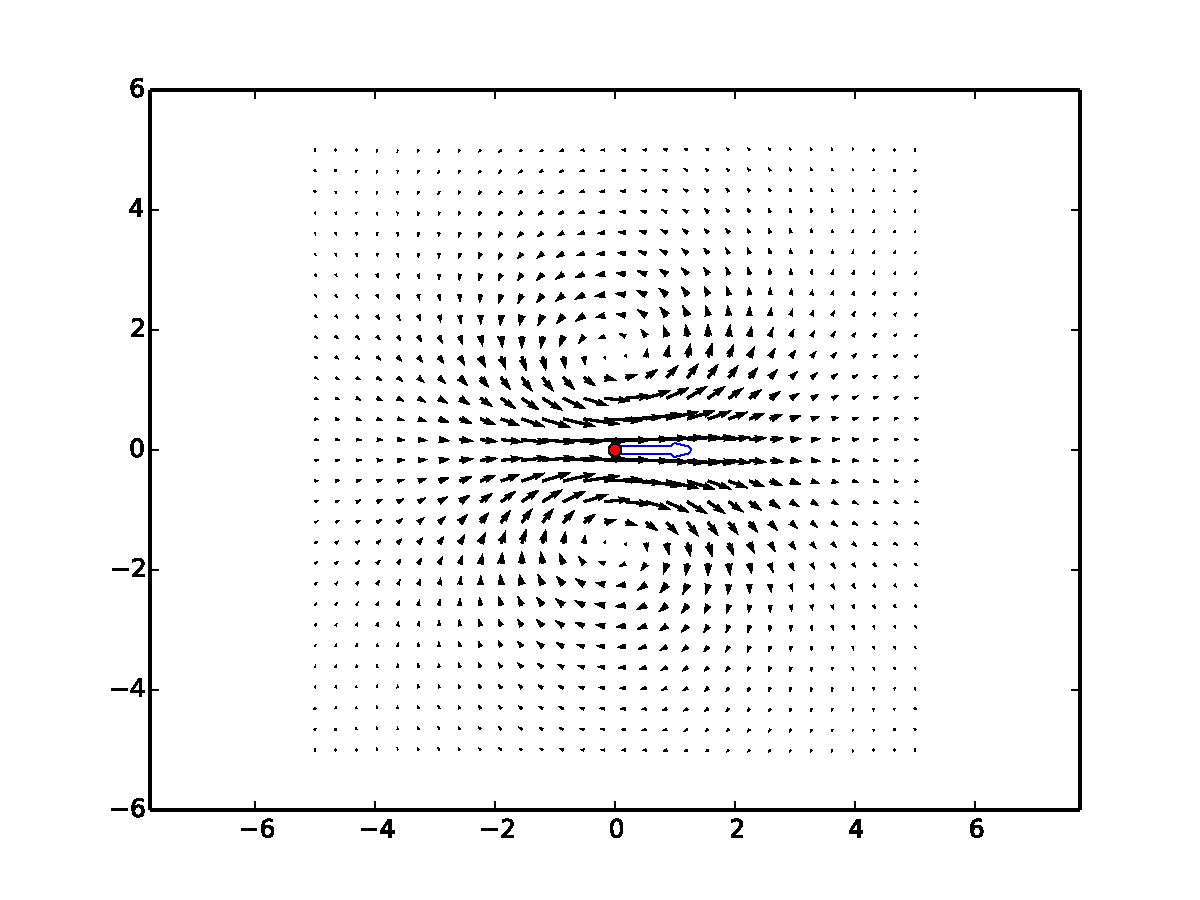
\includegraphics[width = 0.6\textwidth]{./images/zero_jet}
	\caption{A $0$-jetlet with momentum $m = (1,0)^T \otimes \delta_0$.}
	\label{fig:zero_jetlet}
\end{figure}

  Let $z \in Q_N^{(0)}$.
  We can consider the isotropy group $\iso(z) = \{ \varphi \in \SDiff(\R^n) \mid \varphi(z) = z \}$.  The group $\iso(z)$ acts on $Q_N^{(0)}$
  by the trivial right action $q \cdot \varphi = q$.
  This yields the momentum map $J_R^{(0)}(q,p) = 0$.
  We see that $J_L^{(0)}$ is injective, and thus has a trivial kernel.
  As a result, the symplectic orthogonal to the kernel of $J_L^{(0)}$
  is the full tangent bundle $T(T^*Q_N^{(0)})$.
  Moreover, the kernel of $J_R^{(0)}$ is $T(T^*Q_N^{(0)})$ and so its
  symplectic orthogonal is trivial.
  From these observations it follows that the diagram
  \begin{align*}
    \mathfrak{X}_{\rm div}(\R^n)^* \stackrel{J_L^{(0)} }{\longleftarrow}
    T^* Q_N^{(0)}
    \stackrel{J_R^{(0)} }{\longrightarrow} \mathfrak{X}_{\rm div}(\R^n)^* \\
    p_\alpha \otimes \delta_{q_\alpha} \stackrel{J_L^{(0)}}{\longmapsfrom}
    (q,p)
    \stackrel{J_R^{(0)} }{\longmapsto} 0
  \end{align*}
  is a dual pair.
  Again, this dual pair allows us to express conservation
  laws and dynamics as a result of theorem \ref{thm:dual_pairs}.
  The left leg represents the space in which particle-like
  solutions to \eqref{eq:MMDiff} evolve,
  while the right leg represents the conserved quantities
  associated to the trivial symmetry.\je{does this mod out the
    redundancy in the $\SDiff$ action?}
  Specifically, $J_R^{(0)}$ expresses the trivial (perhaps silly)
  conservation law that $0$ is constant in time.
  In summary we find:
  \begin{prop}[\S7 of \cite{MumfordMichor2013}] \label{prop:0-solutions}
  Let $k \geq \frac{n}{2} +1$ and $\sigma > 0$.
  Let $H:T^*Q_N^{(0)} \to \R$ be the function
  \begin{align*}
    H(q,p) =\frac{1}{2} K_{k,\sigma}^{ij}(q^\alpha - q^\beta) p_{\alpha,i} p_{\beta,j}.
  \end{align*}
  If $(q,p)(t)$ is a solution to Hamilton's equations, then
  $m(t) = p_\alpha(t) \otimes \delta_{q^\alpha(t)}$
  is a solution to \eqref{eq:MMDiff}.
\end{prop}
\begin{proof}
	Note that $H = h_{k,\sigma} \circ J_L$ and apply theorem \ref{thm:commuting_actions}.
\end{proof}

\subsection{$1^{\rm st}$-order particle-like solutions}
\label{sec:first_order}
  Let $\SL(n)$ denote the Lie group of $n\times n$ matrices
  with unit determinant.
  Let $q = (q_{(0)}, q_{(1)}) \in \R^n \times \SL(n)$ and consider the left
  $\SDiff(\R^n)$ action on $\R^n \times \SL(n)$ given by
  \begin{align}
    \varphi \cdot q = (\varphi(q_{(0)} ) , D\varphi(q_{(0)} ) \cdot q_{(1)} ). \label{eq:first_order_action}
  \end{align}
  Where $D\varphi(q_{(0)} ) \cdot q_{(1)}$ is the result of multiplying
  the Jacobian matrix $D\varphi(q_{(0)} )$ with $q_{(1)}$.
  \begin{prop}
    The action of $\SDiff(M)$ on $\R \times \SL(n)$ in \eqref{eq:first_order_action} is a group action.
  \end{prop}
  \begin{proof}
    As $\varphi \in \SDiff(\R^n)$, it follows that $D\varphi |_{q_{(0)}} \in \SL(n)$.    Therefore $D\varphi |_{q_{(0)}} \cdot q_{(1)} \in \SL(n)$.
    Secondly, if $\varphi_1,\varphi_2 \in \SDiff(\R^n)$ we observe that
    \begin{align*}
      \varphi_2 \cdot (\varphi_1 \cdot q) &= \varphi_2 \cdot (\varphi_1(q_{(0)} ) , D\varphi_1 |_{q_{(0)}} \cdot q_{(1)} ) \\
      &= (\varphi_2(\varphi_1(q_{(0)} )) , \left. D\varphi_2 \right|_{\varphi_1( q_{(0)} )} \cdot D\varphi_1 |_{ q_{(0)} } \cdot q_{(1)} ) \\
      &= ( (\varphi_2 \circ \varphi_1)(q_{(0)} ) , D( \varphi_2 \circ \varphi_1)|_{q_{(0)} } \cdot q_{(1)} ) \\
      &= (\varphi_2 \circ \varphi_1) \cdot q,
    \end{align*}
    where the second and third line is an application of the chain rule.
  \end{proof}
  As before, this action can be lifted to the cotangent bundle $T^*(\R^n \times \SL(n))$.  In particular, 
  the action is
  \begin{align*}
    &T^*\varphi \cdot ( q_{(0)} , q_{(1)}  , p_{(0)} , p_{(1)} ) \\
    &\quad = ( \varphi^{-1}(q_{(0)})  , [D\varphi|_{q_{(0)}}]^{-1} \cdot q_{(1)} , D\varphi|_{q_{(0)}}^* \cdot p_{(0)} , D\varphi|_{q_{(0)}}^* \cdot p_{(1)} ).
  \end{align*}
  The resulting momentum map is
  \begin{align*}
    J_L^{(1)}( (q, j ),(p, p_j) ) = p_\alpha \delta_{q^{\alpha}} + \dots
  \end{align*}
  \todo[inline]{A David calculation goes in place of ``...''}
  As before, we can generalize this construction to the space of
  $N$-particles by considering the space
  \begin{align*}
    Q^{(1)}_N = \left\{  ( q^1 , \dots, q^N ) \mid 
      \begin{array}{c}
        q^\alpha = (q\indices{^\alpha_{(0)} } ,q\indices{^\alpha_{(1)} } ) \in \R^n \times \SL(n) \\
        q\indices{^\alpha_{(0)}} \neq q\indices{^\beta_{(0)}} \text{ when } \alpha \neq \beta
      \end{array} \right\}. 
  \end{align*}

  Moreover, there is a (non-trivial) right group action by $\iso(z)$ on $Q^{(1)}_N$ given by
  \begin{align*}
    (q_{(0)} , q_{(1)} ) \cdot \psi = (q_{(0)} , q_{(1)} \cdot D\psi|_z).
  \end{align*}
  This action yields the cotangent lift momentum-map
  \begin{align*}
    J_R^{(1)}( q,p) = ....
  \end{align*}
  \todo[inline]{Another one of David's calculations goes above.}
  \begin{prop}
    The momentum maps $J_L^{(1)}$ and $J_R^{(1)}$ form a dual pair.
  \end{prop}
  \begin{proof}
    The actions of $\SL(n)$ and $\SDiff(\R^n)$ on $Q_N^{(1)}$ clearly commute
    and lift to symplectic actions on $T^*Q_N^{(1)}$.
    Moreover, the action of $\SDiff(\R^n)$ is transitive on $\SL(n)$ orbits
    by inspection.
    By theorem \ref{thm:commuting_actions}, $J_L^{(1)}$ and $J_R^{(1)}$ form a dual pair.
  \end{proof}

  As before, the quantity $dh( J_L^{(1)}(q,p))$ is a legitimate vector field
  if $K_{k,\sigma}$ is sufficiently smooth.  Moreover, when the Hamiltonian
  $H^{(1)} = h_{k,\sigma} \circ J_L^{(1)}$ is $C^1$ we may evolve Hamilton's equations
  to obtain solutions.
  
  \begin{prop} \label{prop:1-solutions}
  	If $K_{k,\sigma}$ is $C^{\frac{d}{2} + 2}$ then $H = h_{k,\sigma} \circ J_L$
	is $C^1$ and given by the expression
	\begin{align*}
		H^{(1)}(q,p) = \frac{1}{2} p_{\alpha,i} K^{ij}_{k,\sigma}(q^\alpha - q^\beta) p_{\beta,j}
			+ p_{\beta,j} p \indices{_{\alpha,i}^r} q \indices{^{\alpha,k}_r} \partial_k K^{ij}_{k,\sigma}( q^\alpha - q^\beta) \\
			- p\indices{_{\alpha,i}^r} q\indices{^{\alpha,n}_r} p\indices{_{\beta,j}^s} q\indices{^{\beta,s}_k} \partial_{nk} K^{ij}(q^\alpha - q^\beta).
	\end{align*}
	If $(q,p)(t) \in T^*Q_N^{(1)}$ is a solution to Hamilton's equations with respect to 
	$H^{(1)}$, then $J_L^{(1)}( (q,p)(t)) \in \mathfrak{X}_{\rm div}(\R^n)^*$ is
	a solution of \eqref{eq:MMDiff} and $J_R^{(1)}( (q,p)(t)) \in \mathfrak{X}_{\rm div}(\R^n)$ is
	constant in time. 
  \end{prop}
  The proof of the above proposition is identical to that of proposition \ref{prop:0-solutions}.
  
  Various vector fields for large $k$
  are depicted in figure \ref{fig:zoo}.
  
  \begin{figure}
  	\centering
	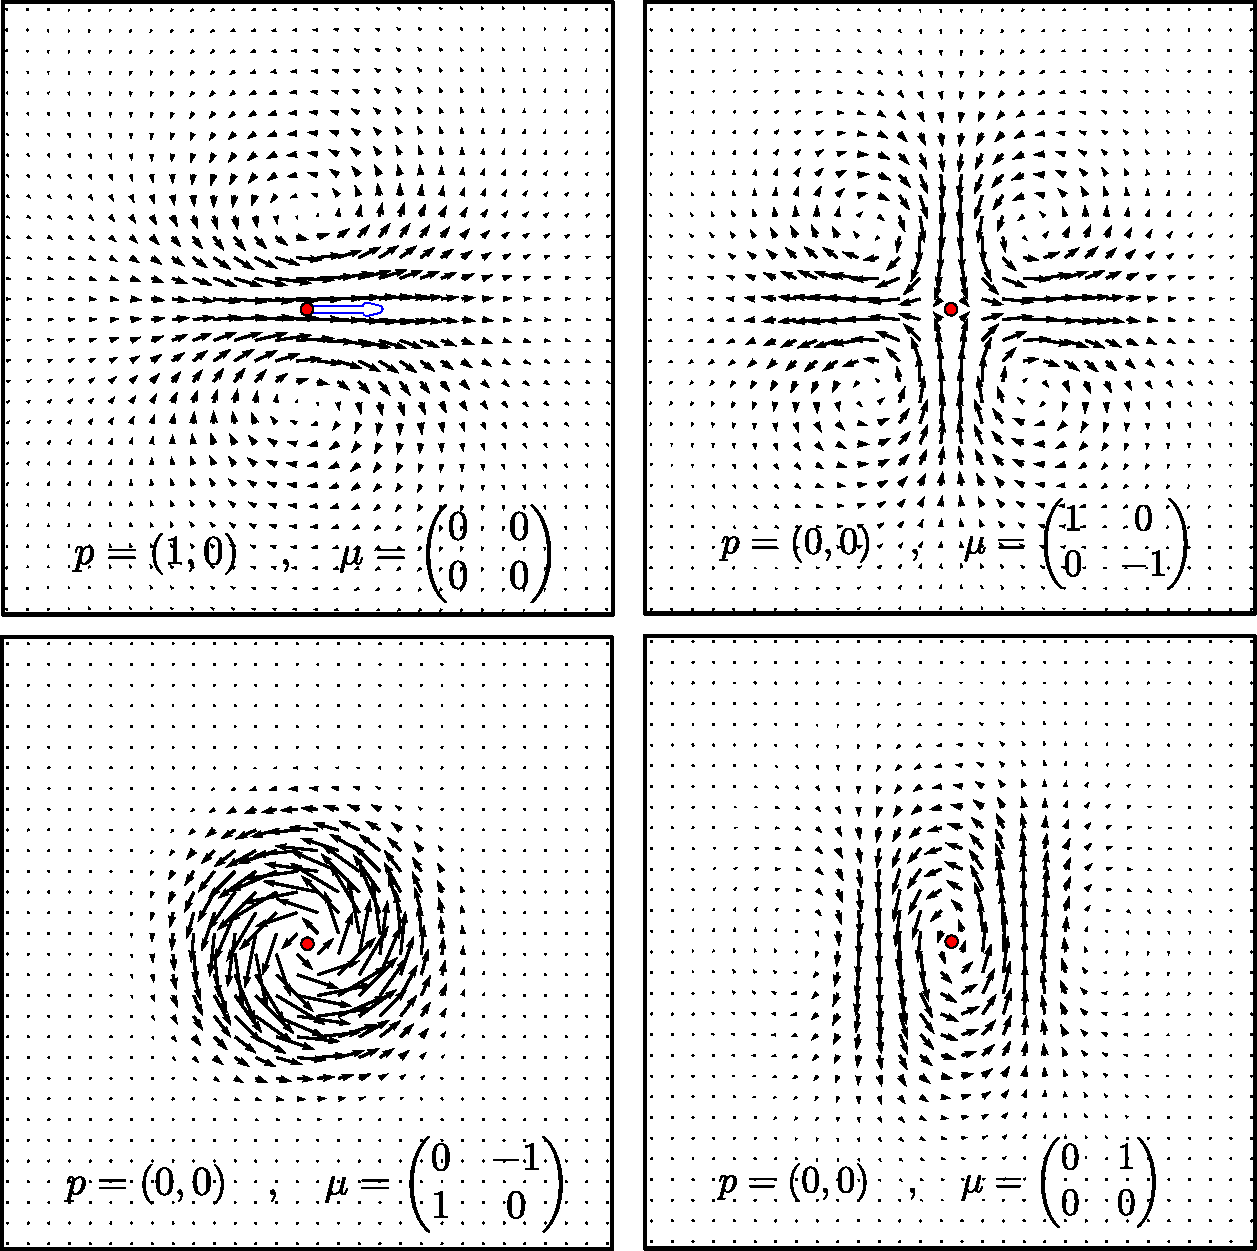
\includegraphics[width=0.5\textwidth]{./images/zoo}
	\caption{a zoo of $1^{\rm st}$-order jet lets}
	\label{fig:zoo}
  \end{figure}

  \subsection{Higher-order particles}
  \label{sec:higher_order}
  In this section we will introduce a hierarchy of particle methods
  where the $k^{\rm th}$ level of the hierarchy includes the $(k-1)^{\rm th}$
  level.
  The $0^{\rm th}$-level in the hierarchy is the standard particle like solutions,
  while the $1^{\rm st}$ level describes particles with internal $\SL(n)$ variables
  mentioned in the previous section.
  These particles in the $k^{\rm th}$-level carry the coefficients of
  $k^{\rm th}$-order Taylor expansions of diffeomorphisms,
  or \emph{jets}.
  Therefore, we call these particles \emph{$k$-jetlets}.

  Let $\varphi \in \SDiff(\R^n)$.
  The zeroth-order Taylor expansion of $\varphi$ about $0$
  is simply $\varphi(0)$, and the collection of such Taylor
  expansions is all of $\R^n$.
  The $1^{\rm st}$-order Taylor expansion of $\varphi$ about $0$ is
  \begin{align*}
    \varphi^i( x) = \varphi^i(0) + \partial_j \varphi^i(0) x^j + o( \|x\|).
  \end{align*}
  The tuple of coefficients $(\varphi(0) , D\varphi(0) ) \in \R^n \times \SL(n)$ is
  called the $1^{\rm st}$-order jet of $\varphi$ evaluated at $0$.
  Going further, the second-order Taylor expansion of $\varphi$ about $0$
  is
  \begin{align*}
    \varphi^i(x) = \varphi^i(0) + \partial_j \varphi^i(0) x^j + 
    \frac{1}{2} \partial_{jk} \varphi^i(0) x^j x^k + o( \| x\|^2).
  \end{align*}
  We see that $D^2\varphi(0)$ is a tensor of rank $(1,2)$, which is
  symmetric in the lower indices.
  We call the space of such tensors $S^1_2$,
  and we see that the space of second-order jets is $\R^n \times \SL(n) \times S^1_2$.
  Finally, for $k \geq 2$ the space of $k^{\rm th}$ order jets is
  \begin{align*}
    Q_1^{(k)} = \R^n \times \SL(n) \times S^1_2 \times S^1_3 \times \cdots\times S^1_k
  \end{align*}
  where $S^1_j$ is the vector space of $(1,j)$-tensors which
  have been symmetrized in the covariant indices.
  The space $Q_1^{(k)}$ is equipped with the fiber bundle
  projection $\pi^{(k)} : Q_1^{(k)} \to \R^n$,
  which simply projects the $\R^n$ component.
  We define the space for $N$-jetlets by taking a product
  \begin{align*}
    Q^{(k)}_N = \{ (q^1,\dots, q^N) \in Q_1^{(k)} \times \dots Q_1^{(k)}
    \mid i \neq j \implies \pi^{(k)}( q^i) \neq \pi^{(k)}( q^j) \}.
  \end{align*}
  We coordinatize $Q^{(k)}_N$ as follows.
  We will use $i,j,k,\dots$ to index particles and Greek indices to indices to represent
  multi-indices on $\R^n$.  A typical coordinate on $Q^{(k)}_N$ will therefore look
  like $q\indices{^{i,\alpha}_{\beta}}$ where $i \in \{1,\dots,N\}$, $\alpha \in \{ 1 , \dots, d \}$
  and $\beta$ is a multi-index on $\R^n$.\todo{Should we elaborate further on multi-indices?
  I'm leaving the multi-index convention to David since he is the one who has to work with it the most.}
  This coordinate is used to model the partial derivative of the $\alpha^{\rm th}$ coordinate
  of a diffeomorphism at some point $z_i$, i.e.\ $\partial_\beta \varphi^\alpha(z_i)$.
  This is the primary motivation for this notational convention.
  We will let $q \indices{^{i,\alpha}_{(k)}}$ denote the collection of $q\indices{^{i,\alpha}_\beta}$
  where $| \beta | = k$.

  \begin{prop}
    The group $\SDiff(\R^n)$ acts on $Q_N^{(k)}$ by a left Lie group
    action.  If $z_1 ,\dots,z_N \in \R^n$ are distinct points,
    then the isotropy group $\iso(z_1,\dots,z_N) \subset \SDiff(\R^n)$
    acts on $Q_N^{(k)}$ by a right Lie group action.
  \end{prop}
  \begin{proof}
    Let $\varphi_1,\varphi_2 \in \SDiff(\R^n)$.
    The partial derivatives of $(\varphi_1 \circ \varphi_2)$
    are given by a formula known as the Fa\`a di Bruno formula
    (see appendix \ref{app:FaadiBruno}).
    One can read directly from the expression that
    a $k^{\rm th}$ order derivative only depends on lower order
    partial derivatives of $\varphi_1$ and $\varphi_2$.
    Let $\Jet^k_z: \SDiff(\R^n) \to Q_1^{(k)}$ denote
    the function which evaluates the $k^{\rm th}$-order
    jet of a diffeomorphism at the point $z \in \R^n$.
    A left $\SDiff(\R^n)$ action is induced on $Q_1^{(k)}$ by
    the setting $\varphi \cdot q = \Jet_z^{(k)}( \varphi \circ \psi)$
    for any $\psi$ such that $\Jet^{(k)}_z(\psi)$.
    That this is independent of the choice of $\psi$ follows
    from observing that the Fa\`a di Bruno formula
    only uses data in $q = \Jet^{(k)}(\psi)$ and nothing more.
    By the same construction, a left $\iso(z)$ action is induced
    on $Q_1^{(k)}$ by setting $q \cdot \phi = \Jet^{(k)}_z ( \psi \circ \phi)$ for any $\psi$ such that $\Jet_z^{(k)}(\psi) = q$.
    We can choose distinct points $z_1,\dots,z_N \in \R^n$
    and easily apply the same process to $Q_N^{(k)}$.
  \end{proof}
  
  Just as in the previous sections, the actions of $\SDiff(\R^n)$ and $\iso(z)$ lift to commuting actions on $T^*Q_N^{(k)}$.
  The associated momentum maps are
  \begin{align*}
    J_L^{(k)} = blah \\
    J_R^{(k)} = blah
  \end{align*}
  \todo[inline]{Another David calculation}
  The action of $\SDiff(\R^n)$ is transitive on $Q_N^{(k)}$,
  and it is therefore transitive on orbits of the right action of $iso(z)$.
  By theorem \ref{thm:commuting_actions}, $J_L^{(k)}$ and $J_R^{(k)}$ form a dual pair.
  Lastly, this gives us the final result on jetlet parametrized solutions.
  The proof is identical to that given in the proposition \ref{prop:0-solutions}.
  \begin{prop}
  	If $K_{k,\sigma}$ is $C^{\frac{d}{2} + 2k}$ then $H^{(k)} = h_{k,\sigma} \circ J_L^{(k)}$
	is $C^1$.
        Let $(q,p)(t)$ be a solution to Hamilton's equations on 
        $T^*Q^{(k)}_N$, then $J_L^{(k)}( (q,p)(t))$ is a solution to Hamilton's
        equations on $\mathfrak{X}_{\rm div}(\R^n)^*$
        and $J_R^{(k)}( (q,p)(t))$ is constant in time.
  \end{prop}
  
  \subsection{Kelvin's circulation theorem}
  \label{sec:Kelvin}
  In this section we relate the conserved quantities associated
  to $J_R^{(k)}$ to Kelvin's circulation theorem.
  \todo[inline]{Darryl, would you like to write this section?  To correspond with [Desbrun Jacobs Ratiu 2013]
  	see Theorem 5.5 of that article.  The quantity ``$J_\omega$'' in that paper is equivalent to our $J_R$.}


\section{Collisions}
\label{sec:collisions}
Analytic analysis of collisions with $j=0$.
Discuss mergers to higher-order, time to collision, near misses.

\todo[inline]{Jaap can write this}

\section{Numerical experiments}
\label{sec:Numerical experiments}

\cjc{Consider two particles, far apart.  Each has it's``own conserved momenta".  They get close, exchange stuff, but the ``actual" momentum is conserved}

\cjc{Collide some $k$-jets.  Make correspondence with total momentum.}


\appendix
\section{Convergence and error bounds}
\label{sec:Convergence}
He we prove that the particle method converges to a solution of the Mumford--Michor model for an arbitrary initial condition in $H^k_{\sigma^2}$.

We cite error bounds to Euler from Mumford--Michor.

\todo[inline]{Not really sure if this section is worth writing.  It follows almost directly from \cite{TrouveYounes2005}.}

\section{Computations with the Fa\`a di Bruno formula}
\label{app:FaadiBruno}

\todo[inline]{A space for David's computations}

\bibliographystyle{amsalpha}
\bibliography{hoj_2014}

\end{document}
